	\documentclass[fleqn, 12pt]{article}
	\usepackage[latin1]{inputenc}
	\usepackage[ngerman]{babel}
	\usepackage[a4paper,text={155mm,220mm},centering,headsep=10mm,footskip=15mm]{geometry}
	\usepackage{graphicx}
	\usepackage{amssymb}
	\usepackage{graphicx}
	\usepackage{multirow}
	\usepackage{multicol}
	\usepackage{float}
	\usepackage{pdfpages}
	\usepackage{todonotes}
	\usepackage{pst-plot}
	\usepackage{pstricks}
	\usepackage{pstricks-add}
	\usepackage{pst-node}
	\usepackage{pst-grad,multido} 
	\usepackage{verbatim}
	\title{}
	\date{}
	\author{}
	\usepackage{array}
	\usepackage{amsmath}
	\usepackage{fancyhdr}
	\usepackage{enumitem} 
	\parindent0pt
	%\usepackage[format=plain, justification=RaggedRight, singlelinecheck=false]{caption}
	\usepackage{blindtext}
	
	% Listings
	\usepackage{listings}
	\renewcommand{\lstlistlistingname}{Liste der Quellcode Ausschnitte}
	\renewcommand{\lstlistingname}{Quellcode Ausschnitt}
		\definecolor{lsgreen}{rgb}{0,.5,0}
		\definecolor{lsred}{rgb}{.7,0,0}
		\definecolor{lsorange}{rgb}{.9,.5,0}
		\definecolor{lsgray}{rgb}{.5,.5,.5}
		\lstset{
			frame=tb,
			aboveskip=10mm,
			belowskip=10mm,
			showstringspaces=false,
			columns=flexible,
			captionpos=b,
			basicstyle={\normalsize\ttfamily},
			numbers=left,
			numberstyle=\tiny\color{lsgray},
			keywordstyle=\color{blue},
			commentstyle=\color{lsorange},
			stringstyle=\color{lsgreen},
			breaklines=true,
			breakatwhitespace=true,
			rulecolor=\color{lsgray},
			xleftmargin=7mm,
			tabsize=3
		}
	
	% Needed for proper display of links in bibliography
	\usepackage{url}	
	
	% Hyperref
	\usepackage[
	pdfauthor={Laura Anger, Timo \dots, Lukas Kolhagen},
	pdftitle={BVA Bewegungsanalyse},
	pdftoolbar=true,	
	colorlinks=true,
	linkcolor=blue,
	citecolor=blue,
	urlcolor=blue,
	linktocpage=true
	]{hyperref}
	\usepackage{bookmark}
	\bookmarksetup{
	numbered
	}
	\urlstyle{same}
	
	\pagestyle{fancy}
	\fancyhf{}
	\fancyhead[LO]{BVA}
	\fancyhead[CO]{Bewegungsanalyse in einer Videosequenz}
	\fancyhead[RO]{\thepage}
	\renewcommand{\headrulewidth}{0.5pt}
	\newcommand{\Absatzbox}[1]{\parbox[0pt][2em][c]{0cm}{}}
	
	% Itemize symbol
	\renewcommand{\labelitemi}{$\triangleright$}
	
	% Colors
	\definecolor{yellow}{rgb}{.95,.85,0}
	\definecolor{green}{rgb}{0,.8,0}
	\definecolor{blue}{rgb}{0,0,.8}
	\definecolor{red}{rgb}{.8,0,0}
	\definecolor{grey}{rgb}{.4,.4,.4}
	\definecolor{orange}{rgb}{.9,.5,0}
	
	% Macro for typesetting C++
	\newcommand{\CC}{C\nolinebreak\hspace{-.05em}\raisebox{.4ex}{\tiny\bf +}\nolinebreak\hspace{-.10em}\raisebox{.4ex}{\tiny\bf +}}
\def\CC{{C\nolinebreak[4]\hspace{-.05em}\raisebox{.4ex}{\tiny\bf ++}}}

\begin{document}
\thispagestyle{empty}
	%\sffamily
			\begin{center}
			
\includegraphics[width=.35\textwidth]{logo_TH}\\[20ex]
			{\Huge\textbf{Projektdokumentation}}\\[8ex]
			\rule{.8\textwidth}{.2pt}
			{\Large Bewegungsanalyse einer Videosequenz\\[1ex] mit dem Ansatz des Papers
			von Aach und Kunz}\\
			\rule{.8\textwidth}{.2pt}\\[10ex]
			von\\[2ex]
			\begin{tabular}{ll}
			Laura Anger &(Matrikelnr. 11086356)\\ 
			Timo Breuer &(Matrikelnr. XXXXXXXX)\\ 
			Lukas Kolhagen &(Matrikelnr. 11084355)\\
			\end{tabular}\\[10ex]
			Durchgef�hrt im\\ \textbf{Master Medientechnologie}\\ im\\ 
			\textbf{Sommersemester 2016}\\			
			\end{center}
			\vfill
			\begin{flushleft}
			{\bf Betreuer:}\\
			Prof. Dr. Dietmar Kunz\\
			Institut f�r Medien- und Phototechnik
			\end{flushleft}
	\newpage
	\tableofcontents
	\newpage
	\section{Einleitung}\todo[inline]{Lukas}
	Diese Ausarbeitung ist Teil der Abschlussprojekt-Dokumentation im Modul "`Weiterf�hrende Themen der Bildverarbeitung"' im Master Medientechnologie an der Technischen Hochschule K�ln.
	
	Das Projekt besch�ftigte sich mit der Bewegungsanalyse einer Videosequenz mit dem Ansatz des Papers von Aach und Kunz\textsuperscript{\cite{aach1998bayesian}}. Es wurde bearbeitet von Laura Anger, Timo Breuer und Lukas Kolhagen.
	\subsection{Ansatz im Paper von Aach und Kunz}
	Die Grundlage f�r das vorliegende Projekt bildet das Paper "`Bayesian motion estimation for temporally recursive noise reduction in X-ray fluoroscopy"'. Dieses besch�ftigt sich mit der Entwicklung einer robusten Methode zur Bewegungssch�tzung f�r die speziellen Anforderungen der stark rauschenden Aufnahmen einer R�ntgen-Fluoroskopie.\\
	Der Ansatz beruht auf der Modellierung drei essenzieller Faktoren:
	\begin{description}
		\item [Datenterm:] Unterschied der Grauwerte zweier aufeinander folgender Bildern.
		\item [�rtliche Koh�renz:] Au�er an Randbereichen von Objekten, bewegen sich Nachbarschaften meist in die gleiche Richtung.
		\item [Zeitliche Koh�renz:] Bewegungen verlaufen normalerweise kontinuierlich, sodass sich ein Bildblock zwischen zwei Bildern wahrscheinlich in dieselbe Richtung weiterbewegt oder die Richtung nur gering �ndert.
	\end{description}
	Eine genaue Beschreibung dieser Faktoren erfolgt in \ref{sec:costFunc}.\\
	
	\subsection{Projektziel}
	Die Zielsetzung f�r das Projekt "`Bewegungsanalyse einer Videosequenz"' war eine �ber\-tra\-gung des Ansatzes von R�ntgenbildern auf normale Videosequenzen. Infolge dessen war eine Vernachl�ssigung der speziellen Anforderung des Bildrauschens m�glich, da R�ntgenbilder -- insbesondere als Teil einer Fluoroskopie -- zum Schutz des Patienten und des medizinischen Personals nur sehr geringe R�ntgendosen enthalten d�rfen und deshalb ein extrem schlechtes Signal-zu-Rauschverh�ltnis aufweisen. Diese Problematik besteht bei normalen Videosequenzen nicht, weshalb f�r die Untersuchung von vergleichsweise geringem und etwa gleich verteiltem Rauschen ausgegangen werden konnte.
	\section{Verfahren}
		\subsection{Bewegungssch�tzung}\todo[inline]{Laura}
		\newpage %Muss sp�ter entfernt werden
		\subsection{Programmablauf}\todo[inline]{Lukas (Hab den gesamten Teil auskommentiert)}
		\begin{comment}
			\begin{figure}[h!]
			\centering
					\begin{psmatrix}[rowsep=0.3,colsep=0.4]
						\rnode{run}{\psframebox[fillstyle=solid,fillcolor=black]{\footnotesize\color{white}public void run(ImageProcessor ip)}}\\
						\rnode{readStack}{\psframebox[linearc=0.05,cornersize=absolute,fillstyle=solid,fillcolor=black!10]{\footnotesize Read data from stack}}\\
						\rnode{initialize}{\psframebox[linearc=0.05,cornersize=absolute,fillstyle=solid,fillcolor=black!10]{\footnotesize Initialize first motion vector field with zero vectors}}\\
						\rnode{forI}{\psframebox[linearc=0.05,cornersize=absolute,fillstyle=solid,fillcolor=black!10]{\footnotesize\texttt{$i=0$}}}\\
						\dianode[fillstyle=solid,fillcolor=red!30]{condStackSize}{\footnotesize$i<$ \texttt{stack size}?}\\[3mm]
						\dianode[fillstyle=solid,fillcolor=red!30]{frameNotZero}{\footnotesize$i\not=$ \texttt{0}?}\\[3mm]
						\rnode{curFrame}{\psframebox[linearc=0.05,cornersize=absolute,fillstyle=solid,fillcolor=black!10]{\footnotesize Set current frame to i}}\\
						\rnode{forJ}{\psframebox[linearc=0.05,cornersize=absolute,fillstyle=solid,fillcolor=black!10]{\footnotesize\texttt{$j=0$}}}\\
						\dianode[fillstyle=solid,fillcolor=red!30]{condIter}{\footnotesize$j<$ \texttt{iterations}?}\\[3mm]
						\rnode{Vn}{\psframebox[linearc=0.05,cornersize=absolute,fillstyle=solid,fillcolor=black!10]{\footnotesize Set current vector field as previous}}\\
						\rnode{forK}{\psframebox[linearc=0.05,cornersize=absolute,fillstyle=solid,fillcolor=black!10]{\footnotesize\texttt{$k=0$}}}\\
						\dianode[fillstyle=solid,fillcolor=red!30]{condNumBlocks}{\footnotesize$k<$ \texttt{number of blocks}?}\\[3mm]
						\rnode{calcAlt}{\psframebox[linearc=0.05,cornersize=absolute,fillstyle=solid,fillcolor=black!10]{\footnotesize Calculate 14 alternatives for block k}}\\
						\rnode{minimizeCost}{\psframebox[linearc=0.05,cornersize=absolute,fillstyle=solid,fillcolor=black!10]{\footnotesize Minimize cost function for alternatives}}\\
						\rnode{addVec}{\psframebox[linearc=0.05,cornersize=absolute,fillstyle=solid,fillcolor=black!10]{\footnotesize Add vector with minimal cost to motion vector field}}\\
						\rnode{updateProgress}{\psframebox[linearc=0.05,cornersize=absolute,fillstyle=solid,fillcolor=black!10]{\footnotesize Update plug-in progress}}\\
						\rnode{genMVF}{\psframebox[linearc=0.05,cornersize=absolute,fillstyle=solid,fillcolor=black!10]{\footnotesize Generate motion vector field visualization for current frame}}\\
						\rnode{addToOutStack}{\psframebox[linearc=0.05,cornersize=absolute,fillstyle=solid,fillcolor=black!10]{\footnotesize Add motion vector field to output stack}}\\
						\rnode{outWindow}{\psframebox[linearc=0.05,cornersize=absolute,fillstyle=solid,fillcolor=black!10]{\footnotesize Generate and display output window}}\\
					\end{psmatrix}
					\psset{arrows=->,nodesep=0pt}
					\ncline{run}{readStack}
					\ncline{readStack}{initialize}
					\ncline{initialize}{forI}
					\ncline{forI}{condStackSize}
					\ncline{condStackSize}{frameNotZero}\nbput{\footnotesize\color{green}True}
					\ncangle[angle=0, linearc=.1]{frameNotZero}{genMVF}\nbput[npos=.15]{\footnotesize\color{red}False}
					\ncline{frameNotZero}{curFrame}\nbput{\footnotesize\color{green}True}
					\ncline{curFrame}{forJ}
					\ncline{forJ}{condIter}					
					\ncline{condIter}{Vn}\nbput{\footnotesize\color{green}True}
					\ncline{Vn}{forK}
					\ncline{forK}{condNumBlocks}
					\ncline{condNumBlocks}{calcAlt}\nbput{\footnotesize\color{green}True}
					\ncline{calcAlt}{minimizeCost}
					\ncline{minimizeCost}{addVec}
					\ncline{addVec}{updateProgress}
					\ncangle[arm=3cm, angle=180, linearc=.1]{condIter}{updateProgress}\nbput[npos=.25]{\footnotesize\color{red}False}
					\ncangle[arm=1.8cm, angle=0, linearc=.1]{condNumBlocks}{condIter}\nbput[npos=.25]{\footnotesize\color{red}False}
					\ncline{updateProgress}{genMVF}
					\ncline{genMVF}{addToOutStack}
					\ncline{addToOutStack}{outWindow}
					\ncangle[arm=2.8cm, angle=180, linearc=.1]{condStackSize}{outWindow}\nbput[npos=.2]{\footnotesize\color{red}False}
			\caption{Programmablauf}
			\label{fig:programmAblauf}
		\end{figure}
\end{comment}		
		
		\subsection{Kostenfunktion}\label{sec:costFunc}\todo[inline]{Alle}
			\subsubsection{Datenterm}\todo[inline]{Lukas}
			\subsubsection{�rtliche Koh�renz}\todo[inline]{Timo}
			\subsubsection{Zeitliche Koh�renz}\todo[inline]{Lukas}
\subsection{Visualisierung}\todo[inline]{Laura}
		
	\section{Auswertung}\todo[inline]{Laura \& Timo}

\subsection{Testmaterial}\todo[inline]{Laura}
Das Verfahren wird an drei unterschiedlichen Bildsequenzen getestet, die im Folgenden Testmaterial 1-3 genannt werden und alle eine Aufl�sung von 256x2656 Pixeln haben. Bei Testmaterial 1 und Testmaterial 2 wurde ein Bild um bekannte Werte in x- und y-Richtung verschoben. Anzumerken ist auch, dass beide Testmaterialien identisch verschoben wurden. Bei Testmaterial 3 kann die Bewegung der zu sehenden Objekte lediglich gesch�tzt werden. Alle Testmaterialien wurden f�r diese Dokumentation aufgenommen bzw. erstellt.\vspace{0.6cm}

\begin{minipage}{0.5\textwidth}
\begin{figure}[H] 
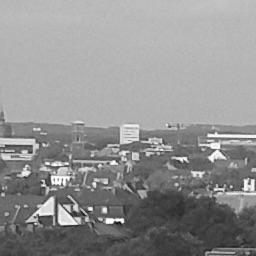
\includegraphics[bb=0 0 256 256, scale=0.77]{Testmaterial1.jpg}
\caption{Standbild Testmaterial 1}
\end{figure}
\end{minipage}
\begin{minipage}{0.5\textwidth}
\textbf{Testmaterial 1}\\
Diese Bildsequenz besteht aus 150 Frames und wurde aus einem Bild der Stadt K�ln erzeugt.\\ 
Bei den ersten und letzten 50 Frames wird ein Ausschnitt des Bildes um jeweils 10 Pixel nach links bzw. oben verschoben. In den mittleren 50 Frames  wird der Bildinhalt um 10 Pixel nach links und 10 Pixel nach unten verschoben. 
\vspace{2.0cm}\\
\end{minipage}\vspace{0.7cm}

\begin{minipage}{0.5\textwidth}
\begin{figure}[H] 
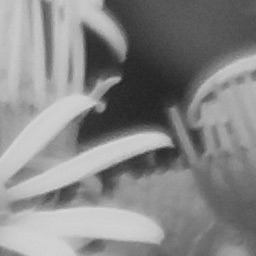
\includegraphics[bb=0 0 256 256, scale=0.77]{Testmaterial2.jpg}
\caption{Standbild Testmaterial 2}
\end{figure}
\end{minipage}
\begin{minipage}{0.5\textwidth}
\textbf{Testmaterial 2}\\
Auf den 150 Frames, die diese Bildsequenz umfasst ist ein Blumenmotiv zu sehen, welches jeweils �ber 50 Frames in verschiedene Richtungen verschoben wird. Auf den ersten Frames erfolgt eine Verschiebung um 10 Pixel nach links. W�hrend die mittleren Frames um sowohl 10 Pixel nach links, als auch 10 Pixel nach oben verschoben wurden, wurde der Bildinhalt der verbleibenden Frames nur um 10 Pixel nach oben verschoben.
\vspace{0.9cm}\\
\end{minipage}\vspace{0.7cm}


\begin{minipage}{0.5\textwidth}
\begin{figure}[H] 
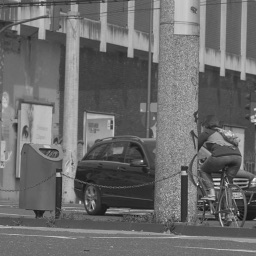
\includegraphics[bb=0 0 256 256, scale=0.77]{Testmaterial3.jpg}
\caption{Standbild Testmaterial 3}
\end{figure}
\end{minipage}
\begin{minipage}{0.5\textwidth}
\textbf{Testmaterial 3}\\
Bei Testmaterial 3 handelt es sich um eine reale Videosequenz, die in K�ln Ehrenfeld aufgenommen wurde. Zu sehen sind ein Auto, dass sich von links nach rechts durch das Bild bewegt und eine Fahrradfahrerin, die das Bild genau entgegengesetzt durchf�hrt. Beide Objekte werden zeitweise durch eine S�ule verdeckt. Die Kamera ist starr, weshalb f�r den restlichen Bildinhalt keine Bewegung zu erkennen ist. Insgesamt besteht die Testsequenz aus 118 Frames.
\vspace{0.9cm}\\
\end{minipage}

		\subsection{Analyse der Kostenfunktion}\todo[inline]{Laura}
		\subsection{Einschwingverhalten}
			\subsubsection{Bewegungsvektorfelder}\todo[inline]{Timo}
			\subsubsection{Innerhalb eines Bildes}\todo[inline]{Laura}
		\subsection{Parameter der Regularisierungsterme}\todo[inline]{Timo}
	\section{Zusammenfassung}\todo[inline]{Lukas}
	\section{Arbeitsaufteilung der Dokumentation}
	\newpage
	\bibliographystyle{plain}
	\bibliography{ABV_Bewegungsanalyse_LaTeX}
\end{document}
		